%-----------------------------------------------------------------------------
%
%               Template for LaTeX Class/Style File
%
% Name:         sigplanconf-template.tex
% Purpose:      A template for sigplanconf.cls, which is a LaTeX 2e class
%               file for SIGPLAN conference proceedings.
%
% Author:       Paul C. Anagnostopoulos
%               Windfall Software
%               978 371-2316
%               paul@windfall.com
%
% Created:      15 February 2005
%
%-----------------------------------------------------------------------------

\documentclass[natbib,10pt,preprint]{sigplanconf}
\usepackage[american]{babel}
\usepackage{graphicx}
\usepackage{hyperref}
\usepackage[table]{xcolor}
\usepackage{listings}
\usepackage{tabularx}
\usepackage{booktabs}
\usepackage[all]{hypcap}        % jump to the picture and not the caption
\usepackage{url}


%%
%% Tune Latex for better usage of white space
%%
\renewcommand{\topfraction}{0.95}
\renewcommand{\textfraction}{0.05}
\renewcommand\floatpagefraction{0.95}
\renewcommand\dbltextfloatsep{12pt}
\renewcommand\textfloatsep{12pt}
\setlength{\abovecaptionskip}{0pt}
\setlength{\belowcaptionskip}{0pt} 
\clubpenalty=0
\widowpenalty=0


%%
%% Setup PDF meta information
%%
\hypersetup{
  pdfauthor={Anthony Gitter, Sven Stork},
  pdftitle={Virtual Application Profiler},
  pdfborder={0 0 0}      %% disable border around links
}


\begin{document}

\conferenceinfo{ }
\CopyrightYear{ }
\copyrightdata{ }


\titlebanner{DRAFT -- do not distribute}        % These are ignored unless
\preprintfooter{short description of paper}   % 'preprint' option specified.

\title{Virtual Application Profiler}


%%
%% setup authors and affiliations 
%%

\authorinfo{Anthony Gitter \and Sven Stork }
           {School of Computer Science \\* Carnegie Mellon University  \\* 5000 Forbes Avenue \\* Pittsburgh, PA 15213, USA}
           {\{agitter,svens\}@cs.cmu.edu}


\maketitle

%%======================================================================
%% Introduction
%%======================================================================
\begin{abstract}
As hardware grows more complex and with the transition
to multicore systems, it becomes increasingly important
for software developers to understand the interactions
between their software and the underlying architecture
in order to maximize performance and ensure correctness.
We present the Virtual Application Profiler, a replay
and analysis tool that facilitates this understanding
by allowing programmers to iteratively simulate application execution
on many architecture configurations and evaluate
memory usage and protection in parallel programs.  Our profiler
is unique in that it logs all application execution traces
in a SQLite database, which allows developers to view and
manipulate the logged data with ease.
\end{abstract}



\terms
profiling

\keywords
profiling concurrency simulation


%%======================================================================
%% Introduction
%%======================================================================
\section{Introduction}
The Virtual Application Profiler (VAPP) was designed to give programmers
greater understanding and control of their code in response to
the rising complexity in architecture over the past decades.
In this context, architecture complexity refers to both the
complicated hardware units of a single core (such as the Pentium 4)
as well as the new challenges brought forth by the rise of
multicore machines.

Specifically, our goals are to (1) allow programmers to quickly
simulate application execution over a large set of architecture
configurations, (2) assist in the testing and debugging of
programs that run on parallel architecture, and (3) do so in a
transparent manner that allows programmers to easily access and
query those aspects of an application's behavior that are relevant to
these tasks.  To achieve these goals, we have pursued a software-based
log-and-replay approach, in which a trace of application's execution
is stored and subsequently replayed on simulated architecture or
used for other high level analysis.  The logged data is stored
in a manner that allows the programmer to directly inspect or
make custom inquiries over the trace.

Because VAPP's broad goals encompass replay on simulated architecture
and data race detection, there a large body of related work.
However, similar approaches focus on only one of these two problems.
MemSpy \cite{martonosi1992memspy}, like VAPP, is a software-based
profiler designed to help developers target performance bottlenecks 
due to the memory hierarchy.  MemSpy performs more detailed analysis
than what VAPP presently offers and reports statistics (such as
memory stall time) at the level of code-data pairs.  For instance,
it can show how many stalls are due to memory accesses to a particular
matrix in a specific inner loop of a program.  Unlike VAPP, MemSpy
performs all analysis dynamically, must be rerun every time
the simulated architecture's parameters are changed, and does not
concern itself with parallel program correctness.
SIGMA \cite{derose2002sigma} is more similar to VAPP in that it
instruments code, stores an execution trace, uses the trace
to simulate execution on various hardware configurations, and
logs statistics for the user to view.  It is also software-based
and allows users to simulate execution on many architecture
configurations from a single trace file.  SIGMA is also more
fully featured than VAPP's simulated replay at the moment because it simulates
a larger portion of the memory hierarchy, but it does not target
issues related to data races and parallel program debugging.

Related work relevant to VAPP's second goal includes
data race detectors and deterministic replay tools. 
RecPlay \cite{ronsse2000non} is a software tool
that detects data races by making multiple executions of
the target program, performing different levels of
analysis with each pass.  This enables it to trace
a minimal amount of information as opposed to all memory
accesses.  VAPP only requires an application to be
executed once, and is suitable for more general
parallel program analysis than data race detection.
Eraser \cite{savage1997eraser} is also software-based
and implements a very similar locket algorithm to
detect inconsistent lock usage in parallel programs.
It performs dynamic analysis as opposed to VAPP's
log-and-replay approach, and it limited to analysis
of Pthreads locks unlike VAPP, which also supports
OpenMP.  BugNet \cite{narayansamy2005bugnet} and FDR
\cite{xu2003fdr} both log program execution in order
to replay it in a deterministic manner to assist
in debugging following a crash.  They create checkpoints
of system state and then track all execution for a fixed
window (e.g. 1 billion instructions).  These methods
both require hardware support.  FDR supports full system
replay, whereas BugNet (like VAPP) focuses on user-level
application code only.  BugNet is unique in that it
primarily records only loads, and can reconstruct
deterministic replays from the load data and checkpoints.
However, both FDR and BugNet do not detect data races
or concurrency bugs unless they cause an application
or system to crash.  They also can only replay a fixed
window of execution, unlike VAPP which aims to
replay the entire execution.  Nevertheless, these
two methods support a much more comprehensive form of replay
than VAPP in its current state.
All of the above methods differ from VAPP in that they
only consider a single architecture configuration during
replay and analysis.  Please see Xu et al. \cite{xu2003fdr} for a more
comprehensive comparison of related data race detection
and deterministic replay tools.

Note that none of these methods allow users to access or
query information concerning application execution and behavior
as VAPP does.  Thus, our third goal is one of the primary novel
technical contributions of this
work that distinguishes our approach from the multitude of
related profilers and replay tools.  Unifying our first and
second goals in a single tool is another unique aspect of VAPP,
and to our knowledge all existing related work concentrates on 
only one these two problems that result from architecture-complexity.

We have released VAPP as an open source project, and it is available
for download from our Google Code page (\url{http://code.google.com/p/vapp/}),
which is linked from our project web site.


%%======================================================================
%% Design
%%======================================================================
\section{Design}

\begin{figure}
  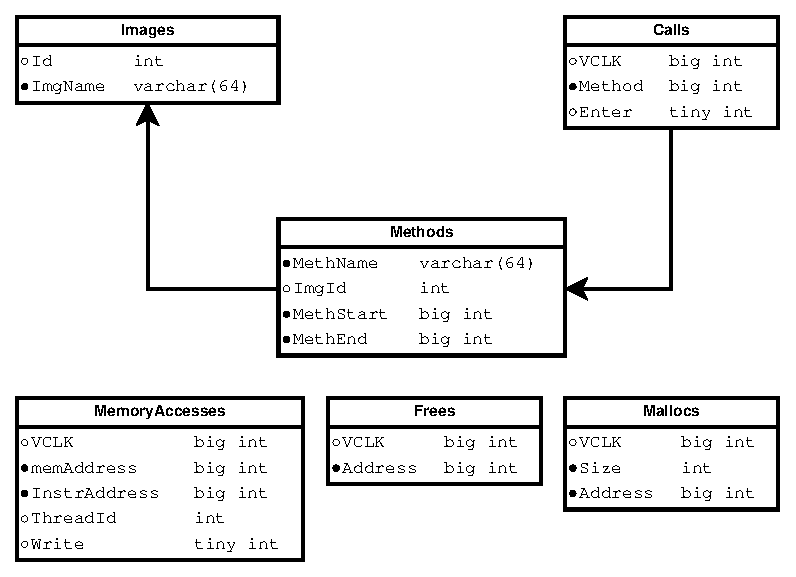
\includegraphics[width=\columnwidth]{database_schema1}
  \caption{Database Schema Pin-Tool1}
  \label{pic:db_schema1}
\end{figure}


\begin{figure}
  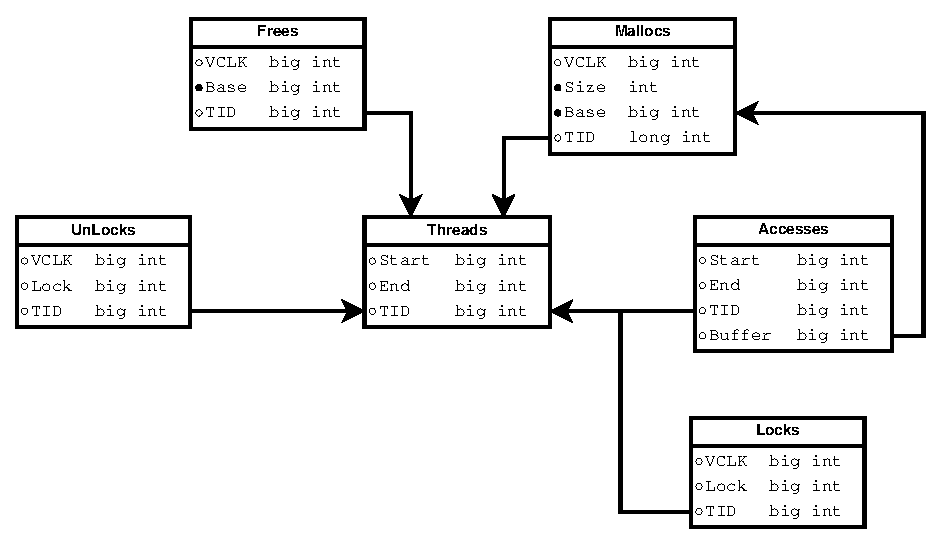
\includegraphics[width=\columnwidth]{database_schema2}
  \caption{Database Schema Pin-Tool2}
  \label{pic:db_schema1}
\end{figure}



%%======================================================================
%% Experimental Setup
%%======================================================================
\section{Experimental Setup}
For our evaluation we used the latest version of the Pin tool
infrastructure available (i.e. pin-2.7-29972). Unless otherwise
specified, all example programs have been compiled with GCC compiler
version 4.4.1, enabling debug information and disabling any
optimizations. We used SQLite version 3.6.16 that was part of our
default Linux distribution.

The benchmarks have been run on an Intel Core2 Quad Q6600 CPU system
with 4GB of main memory, using the software packages described in the
previous paragraph.



%%======================================================================
%% Experimnetal Evaluation
%%======================================================================
\section{Experimental Evaluation}
Compare with FDR, which claims 2\% slowdown in a typically scenario
and 34 MB log files (for 1 billion instruction replay window)
per processor in addition to a full memory dump.

Compare with BugNet, whose First Load Log grew to ~100 MB in the worst
case and less than 20 MB on average when using a window of 1
billion instructions.

Compare with Eraser.  Programs run 10 to 30 times slower with Eraser.

SIGMA does not report slowdown caused by instrumentation, but shows
that some of its logs can grow to hundreds of MB even \emph{after} compression.
However, in other cases a several hundred MB trace is compressed
to a less than 1 MB trace.

MemSpy results in 22 to 58 times slowdown during testing on a single processor.


%%======================================================================
%% Lessons Learned
%%======================================================================
\section{Lessons Learned}
One surprise we encountered relatively early in the project
was the drawbacks of using a SQLite database to store the
application traces.  Our testing showed explosive growth
of the log file size as we scaled our test programs,
with some log files growing to several hundred megabytes
even on moderate length programs.  In addition, as
seen in Section \ref{sec:sim_perf} writing to the database is a
huge bottleneck in the performance of our Pin tool.
While we maintain that may not be a critical problem if the
user intends to amortize the initial cost of creating the
trace over a very large number of simulated replays,
the number of replays required to make the initial instrumented
execution worthwhile is much greater than we expected.  Even then
we need to reduce the I/O costs, because as seen in Table
\ref{tbl:results} the amortization approach fails if
a single execution of the dynamic simulator is faster than
an identical simulation that reads from a trace file.
This suggests
that the reason previous work has not exposed the logged data to
the user to the degree we do is that doing so is impractical
with regard to log file size and exaggerated slowdown.  Commonly
used compression techniques would help reduce I/O costs and log
size, but at the expense of the user's ability to interpret
the stored trace.

Another unexpected challenge we faced during development was
the difficulty in simulating hardware.  As a 125\% goal we
had hoped to simulate more than just the cache, and had considered
using VAPP to demonstrate the effects of using huge page tables
in a system.  However, we were unable to complete this task and
we now understand how daunting it would be to further develop
VAPP to realistically simulate a variety of real architectures and
configurations of those architectures.


%%======================================================================
%% Conclusion and Future Work
%%======================================================================
\section{Conclusions}
Modern systems present an overwhelming array of decisions to
application developers who wish to optimize the architecture 
configuration for their application.  Simultaneously, the
rise of multicore machines and parallel architectures has
further complicated this landscape, and the shift to a parallel
paradigm brings forth new issues pertaining to both performance
and correctness.  To facilitate application development in this
context, we have developed VAPP, a profiling, replay, and analysis tool that 
requires no hardware support and can assist in simulating
program execution on different architecture configurations and
evaluating parallel programs.  VAPP stresses transparency, and
all logged execution traces can be easily accessed and queried
by users.

We have demonstrated VAPP's ability to log detailed memory operations,
lock usage, actions of multiple threads, and function calls.  By
storing logs in a SQLite database, users can view all logged data,
query the log with standard SQL queries, and implement custom
low-level analysis with the queries.  The VAPP replay library
facilitates loading the database and simulating program execution
on the desired architecture.  For parallel programs executing on multiple
cores, VAPP can discover unsafe locking, lock usage, and memory
buffers accessed exclusively be a single thread.  We consider this
project to be a success and feel that we have satisfied our 100\%
goals as well as a one of our 125\% goals, lockset verification.
Work was split TODO: assign distribution of total credit.

While our decision to pursue the goal of trace accessibility may
ultimately prevent VAPP from scaling to operate on real-world
applications due to the size of the log files, we nevertheless
believe this area of the profiler and replayer
design space was under-explored and our pursuit was worthwhile.
Furthermore, by taking a log-and-replay approach instead of
simulating the target architecture during application execution
as is done in some related tools, VAPP is ideal for developers
who intend to simulate one particular execution trace many
times on different architecture configurations.  Conversely,
VAPP is not as well-suited for applications that run on new
input with every modification to the target architecture.  It will
still function in such cases, but the overhead may make it a less
attractive than alternatives that perform simulation alongside
application execution.  One limitation of VAPP is inherent in
dynamic analysis tools for correctness in parallel programs and
as such cannot be easily overcome.  That is, a dynamic tool
can only detect concurrency bugs that occur during program
execution and cannot guarantee that failure to detect such
bugs means they will not arise under different conditions.

Now the we have implemented the core VAPP framework and basic
replay and analysis functionality, there are many directions
for possible future work.  If VAPP is to become competitive
with related profiling and simulation tools, the size of the
log files when tracing medium to large scale programs must be
addressed.  Our control library to dynamically disable logging
during certain parts of execution is a step in the right direction,
but does not help when the programmer wishes to store and replay
a full trace.  Previous approaches for reducing the amount
of data that must be logged, such as Netzer's transitive
reduction \cite{netzer1993optimal}, can likely be introduced to
VAPP or custom compression techniques could be developed.  In addition,
VAPP currently bases all of its analysis on a single logged
execution trace, but since the logs in a database it is feasible
to construct more sophisticated forms of analysis that span multiple
executions.  This would enable programmers to study how features
of the underlying architecture affects performance in ways that
are dependent on the input data or control flow.

We believe that expanding VAPP to provide more rich feedback to
developers of parallel applications is the most exciting prospect
for future development.  VAPP is already able to analyze how
threads use shared memory, and a natural next step would be to
feed such information back to the hardware.  Set pinning in
shared caches in multiprocessors as well as Non-Uniform Memory Architecture
systems could benefit from such feedback by localizing data
to the processors that use it.  Another form of feedback
that could be very to the compiler or hardware would be calculating
lock contention statistics from the already tracked log usage patterns.
This would allow the system to use simple locks for very low contention
locks and more space-intensive or complex locks (e.g. queue-based 
or list-based locks) only as needed.  However, because VAPP analysis
is done offline, one would either need to assume that multithread
memory usage patterns do not significantly vary from execution to
execution or that trends could be generalized by running VAPP on
traces from multiple executions.  

It would also be very interested to reunite our two Pin tools
so that users could replay parallel programs.  Deterministic
replay is an important area of research, and although VAPP does not
presently does not track parallel execution at the same level as
other (hardware-assisted) approaches \cite{narayansamy2005bugnet},
replaying execution based on the order in locks are acquired and
released would provide some form of deterministic replay.  As with
the aforementioned feedback mechanisms, the data needed for such a
feature is already logged and available, which suggests such an
extension would indeed be feasible.


%%======================================================================
%% References
%%======================================================================
\bibliographystyle{plainnat}
\bibliography{references}

\end{document}

